\section{RC Week 9}
\subsection{Sub-types, Code Reuse and Inheritance}
\begin{frame}{Principals of Object Oriented Programming}
There are 5 widely accepted principles throughout the object oriented design:
\begin{enumerate}
	\item \alert{S}ingle responsibility principle
	\item \alert{O}pen/close principle
	\item \textbf{\alert{L}iskov substitution principle}
	\item \alert{I}nterface segregation principle
	\item \alert{D}ependency inversion principle
\end{enumerate}
\begin{itemize}
	\item The idea of ``abstract data type" by first proposed by Barbara Liskov and Stephan Zilles (1974) in  "Programming with abstract data types".
	\item Later on in Liskov's 1988 key note ``Data Abstraction and Hierarchy", the SOLID principles of object oriented programming was first proposed. 
\end{itemize}
\end{frame}
\begin{frame}{Principals of Object Oriented Programming}
\begin{columns}
\column[]{.6\textwidth}
Barbara Liskov (1939 to present)
\begin{itemize}
	\item MIT computer scientist
	\item Ford Professor of Engineering
	\item One of the American's first women PH.D. in Computer Science
\end{itemize}
\column[]{.4\textwidth}

	\vspace{-.15in}\hspace{-.18in}
	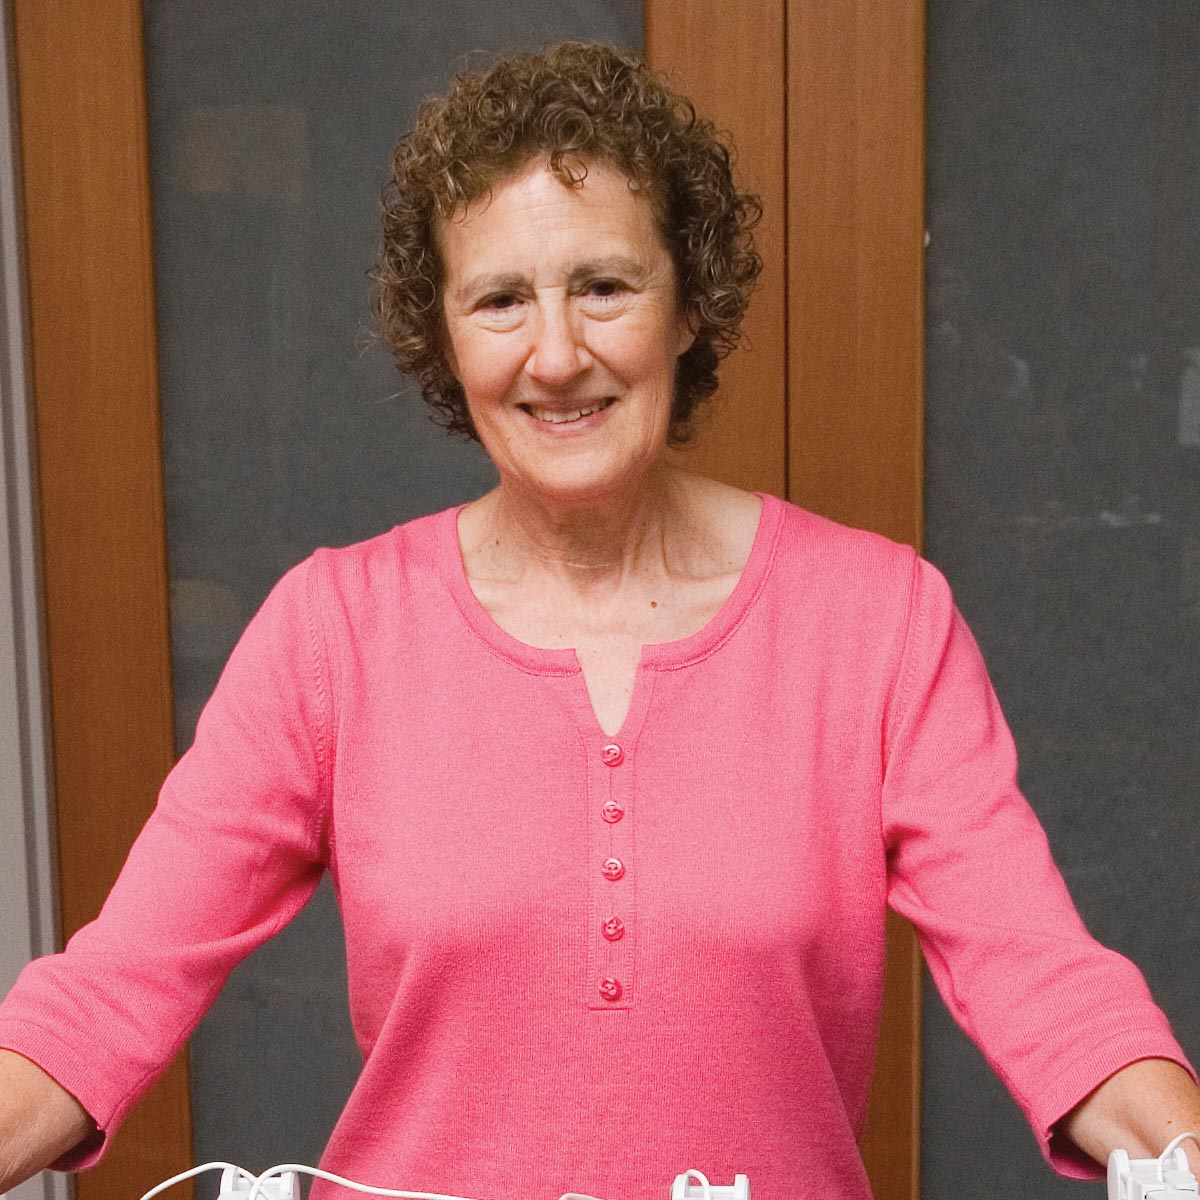
\includegraphics[scale=0.08]{fig/barbara-liskov}

\end{columns}
\begin{itemize}
	\item 2004 John von Neumann Medal winner for "fundamental contributions to programming languages, programming methodology, and distributed systems"
	\item 2008 Turing Award winner, for her work in the design of programming languages and software methodology that led to the development of object-oriented programming
\end{itemize}
\end{frame}

\begin{frame}[allowframebreaks]{Sub types and Liskov Substitution Rule}
The substitution rule is formally described as follows:
\begin{center}
 If $S$ is a subtype of $T$, then objects of type $T$ may be replaced with objects of type $S$ (i.e. an object of type $T$ may be substituted with any object of a subtype $S$) without altering any of the desirable properties of $T$ (correctness, task performed, etc.)
\end{center}
This is by all means very abstract. We provide a more "concrete" explanation.

\begin{center}
	\structure{Subtype relation is an ``IS-A" relationship.}
\end{center}

For examples, a \texttt{Swan} \alert{is a} \texttt{Bird}, thus a \texttt{class Swan} is a subtype of \texttt{class Bird}. A bird can fly, can quake and can lay eggs. A swan can also do these. It might do these better, but as far as we are concerned, we don't care. \texttt{Bird} is the super-type of the \texttt{Swan}.
\end{frame}

\begin{frame}{Pre-conditions \& Post-conditions}
The term ``sub-type" is misguiding because the prefix ``sub" suggests the sub-type is ``inferior" to the super-type in some sense. But this is actually other way around. 

\begin{itemize}
	\item The assertions in the \texttt{REQUIRES} clause and argument types in abstraction specs combined is called a ``Precondition".
	\item The assertions in the \texttt{EFFECTS} and \texttt{MODIFIES} clause specifies the post conditions. 
\end{itemize}

Sub-types typically perform a combination of belows:
\begin{itemize}
	\item Supports extra operation. Naturally preserves follows LSR.
	\item Weakens the pre-conditions. Expands range of input.
	\item Strengthens the post-condition. Enhances the effect.
\end{itemize}
In reality sub-types are beefed-up versions of the super-type. They perform more specific jobs or do the same job better.
\end{frame}

\begin{frame}{Is it a subtype?}
Designing whether something is or is not a subtype of a particular super type is probably in the heart of program structure design.

\structure{A Remark}

The problem of whether two objects form a ``IS-A" relation must be understood in a realistic context. Consider two classes \texttt{RegularIntSet} and \texttt{SortedIntSet}. Suppose both of them supports a \texttt{max()} function.
\begin{itemize}
	\item You can argue that \texttt{RegularIntSet} is a sub-type of \texttt{SortedIntSet} because they support the same set of operations.
	\item You can also claim that\texttt{RegularIntSet} is NOT a sub-type since the \texttt{max()} of \texttt{RegularIntSet} is significantly slower than it's counterpart. One could argue the performance is part of the abstraction.
\end{itemize}
\end{frame}


\begin{frame}{Differentiating \texttt{IS-A} and \texttt{HAS-A}}
Suppose we have a \texttt{class Graph} that abstracts the concept of a graph. It supports \texttt{Graph::InsertNode(string name)} and \texttt{Graph::addEdge(string node1, string node2)}. Suppose we have a class \texttt{Binary} tree that inherits \texttt{Graph}. It supports one more operation \texttt{Tree::GetRoot()}. The question is whether \texttt{Tree} is a sub-type of \texttt{Graph}?
\end{frame}

\begin{frame}{Differentiating \texttt{IS-A} and \texttt{HAS-A}}
Unfortunately the answer is negative. The reason should be obvious. There is essentially no requirement on where the edges and nodes are (precondition is weak). But you can't add arbitrary edges and nodes must connect to at most 2 other nodes (stronger precondition). \alert{So a \texttt{Tree} is not a  \texttt{Graph} in the subtype sense}.

\vspace{0.1in}
However we would naturally see that a \texttt{Tree} type must have a lot common code as the \texttt{Graph}. We would like to avoid rewriting them. There are two ways to do this:
\begin{itemize}
	\item Through \texttt{private} inheritance (implementation inheritance). We would not discuss this.
	\item By setting \texttt{Graph} as a member of a \texttt{Tree} type. We forward calls to \texttt{Graph}. This is a typical case of a \texttt{Has-A} implementation.
\end{itemize} 
\end{frame}


\begin{frame}{Solving the inheritance problem}

\end{frame}
